\secnumbersection{Marco conceptual}

Los algoritmos basados en la técnica Octree deben gestionar el problema mencionado en la sección anterior, la representación incorrecta de los límites del dominio, por sobre todo en dominios cóncavos.

Un octante límite es aquel que intersecta la frontera de $\Omega$ \footnote{$\Omega$ : dominio de entrada para el que se requiere generar una malla.}, puede presentar nodos dentro y fuera del dominio $\Omega$, los nodos que estén justo en la frontera son considerados nodos externos.

Cuando el octante límite contiene sólo un hexaedro, puede emplearse un patrón de superficie, definidos en \cite{lobos2013patterns}, dicho trabajo presenta un conjunto de patrones de elementos mixtos, que se emplean en la superficie del dominio objetivo y permiten conservar la consistencia de las mallas resultantes, estos patrones están pensados para combinarse con cualquier técnica de mallado que produzca una malla hexaédrica regular o irregular, las mallas Octree son un tipo de malla hexaédrica. Un patrón de superficie es un conjunto de diferentes tipos de elementos que sustituyen al hexaedro para reducir las posibilidades de producir elementos inválidos. Dependiendo de la configuración de nodos internos/externos del octante, se empleará un patrón distinto.

En \cite{lobos2015mixed} se describe una técnica de mallado que incluye patrones de superficie y transición. Esta técnica permite definir diversos $RL$ para $\Omega$. Esta técnica es la base del trabajo desarrollado por Daines y Lobos en \cite{daines2018repairing} y del presente trabajo.

En \cite{daines2018repairing} se detectó que este algoritmo puede producir algunos elementos no válidos cuando las transiciones entre regiones de diferente $RL$ se presentan en el borde. Se trata de un octante que debe llenar ambas regiones, gestionar una transición y, al mismo tiempo lograr la representación del borde. 

\subsection{Medida de calidad para elementos en Mallas Mixtas}

En general, la calidad de un elemento geométrico viene determinada por el nivel de deformación en comparación con la representación geométrica más regular o perfecta del elemento.

La medición de la calidad tiene dos propósitos fundamentales: 

\begin{itemize}
	\item Comparar la malla, ya sea con otras mallas producidas por el mismo dominio o con la propia noción de malla ``teóricamente perfecta".
	\item Mejorarla, es decir, obtener una malla ``mejor" comenzando por un estado de mala calidad mediante el uso de algoritmos de reparación.
\end{itemize}

% Para el hexaedro, el tetraedro y la cuña se utiliza la variación regular. Por desgracia no existe una variación regula para todas las pirámides. 

Existen múltiples medidas de calidad de los elementos geométricos utilizados, cada una de las cuales mide distintos tipos de deformaciones.
Una medida utilizada habitualmente es la relación de aspecto, $AR$ \footnote{ AR : Aspect Relation.}. En general, el $AR$ de un elemento es la relación entre su borde más corto y su borde más largo. Otra variación significativa es el Relación de Aspecto Gamma, ARG \footnote{ARG: Aspect Ratio Gamma.}, el $ARG$ penaliza más las deformaciones de un tetraedro en comparación con otras variaciones del $AR$.
Para medir la distorsión de un nodo en contraste con su vecino podemos utilizar la \textit{Jacobiana}. Siendo $J^a$ el Jacobiano del nodo $a$ y $d_i$ el vector del nodo $a$ al nodo $i$. El Jacobiano se puede calcular realizando el producto punto entre la distancia nodal del vector altura del tetraedro y el producto cruz de las distancias nodales de los vectores basales.

El problema del Jacobiano es sus dependencias a las distancias entre nodos y a la ortogonalidad entre sus aristas, con respecto a la primera, dos elementos con los mismos ángulos internos pero con tamaños distintos de aristas obtienen distintos valores para esta medida de distorsión y sobre la segunda, la medida de calidad no se puede extender a todos los tipos de elementos geométricos que se encontrarán en este tipo de mallas, mallas mixtas.

Por tanto, para suplir la dependencia a las distancias se utilizará el Jacobiano Escalado, $J_S$ \footnote{$J_S$ : Scaled Jacobian}.
Esta medida de calidad normaliza los vectores del tetraedro, así sólo dependerá de la ortogonalidad de sus aristas.
El $J_S$ de un hexaedro es el peor $J_S$ de sus nodos. 

En \cite{daines2018repairing} se define el rango de aceptación de la calidad de los elementos. Principalmente, $J_S < 0$ son Elementos invertidos, se define en \cite{shepherd-2008} un estándar utilizado en las métricas de calidad para Jacobiano Escalado importado por la librería Veredict de Cubit \cite{verdict} que fija $J_S < 0$ como Elementos de inaceptables y $J_{S} \in [0, 0.2[$, correspondería a Elementos cuestionables, es decir, Elementos de calidad deficiente. Además, se destaca el estándar de ANSYS, una herramienta robusta a la hora de realizar simulaciones computarizadas, que considera $J_{S} \in [0, 0.03[$, como Elementos inválidos. Elementos con $J_S \geq 0.2$ como Elementos de buena calidad y Elementos con $J_{S} = 1$, como un hexaedro perfecto.

%
Por tanto, para este análisis se acotará definiendo $J_{S} \in ]-\infty, 0]$ como Elementos inválidos, estos específicamente corresponden a Elementos negativos o invertidos, que conformarían mallas con topología inconsistente. Luego, se considerará, a diferencia de los trabajos anteriores, Elementos de calidad cuestionable los que presenten $J_{S} \in ]0, 0.05]$, este intervalo se acotará y separará en dos intervalos, $J_{S} \in ]0, 0.03] \wedge J_{S} \in ]0.03 , 0.05]$, esto con el fin de enfocar el estudio en Elementos que produzcan una malla inconsistente, reduciendo la cota superior de $0.2$ a $0.05$ y estudiar las consecuencias en la propagación del cambio de la calidad del refinamiento, dividiendo el intervalo en dos, considerando el estandar de ANSYS como referencia al dividir dicho intervalo.

%Además, se definirá la frecuencia de Elementos con $J_{S} \in ]m, n]$ , como $E^{n}_{m}$.
%
%Entonces, se graficará en \autoref{fig:fit_all_bar}, los histogramas de cada malla para los intervalos definidos por $EC$.
%Teniendo, $E^{0}_{-inf}$, $E^{0.03}_{0}$, $E^{0.05}_{0.03}$, como los intervalos a estudiar, en $E^{0}_{-inf}$ se refleja la cantidad de Elementos por refinar en cada iteración, analizado anteriormente en el ajuste.
% Más adelante se establecerán diferentes estandares para identificar elemementos inválidos


Por otra parte, para suplir la deficiencia en su dependencia a la ortogonalidad de sus aristas, se usará un Jacobiano para cada uno de los tipos de elementos que encontraremos en la malla, esta medida de calidad es el Jacobiano Escalado Normalizado del Elemento \footnote{$J_{ENS}$ : Element Normalized Scaled Jacobian}, más adelante denotado como $J_{ENS}$.


El indice $J_{ENS}$ calcula el $J_S$ del elemento perfecto $K^e$, donde $e$ denota el elemento correspondiente. Los valores para los distintos elementos utilizados en este trabajo para las mallas Octree mixtas se encuentran en la siguiente \autoref{eq:const_jens}.


\begin{equation} \label{eq:const_jens}
    \begin{aligned}
    K^T &= \frac{\sqrt{2}}{2} \longrightarrow \text{Tetraedro} \\
    K^P &= \frac{\sqrt{6}}{3} \longrightarrow \text{Pirámide} \\
    K^W &= \frac{\sqrt{3}}{2} \longrightarrow \text{Cuña}
    \end{aligned}
\end{equation}

De esta forma, como se vio en \cite{daines2018repairing}, con ayuda de estas constantes podemos calcular el $J_{ENS}$ de cualquier nodo de un elemento sustituyendo el valor correspondiente en la \autoref{eq:node_jens}. De forma similar a $J_S$ para realizar el cálculo de $J_{ENS}$ utilizamos la \autoref{eq:jens}, donde $i$ son los nodos del elemento $e$. y $J^e_{ENS}$ es su $J_{ENS}$.

\begin{equation} \label{eq:node_jens}
    \begin{aligned}
J^n_{ENS} &=    
\left\{
\begin{array}{rl}
     ( 1 + K^e ) - J_S, & \qquad J_S > k^e
  \\ Js/K^e, & \qquad -k^e \leq J_S \leq K^e
  \\ -( 1 + K^e ) - J_S, & \qquad J_S < -k^e
\end{array}
\right.
    \end{aligned}
\end{equation}


\begin{equation} \label{eq:jens}
    \begin{aligned}
J^e_{ENS} &=    
\left\{
\begin{array}{ll}
     \text{min}\{J^i_{ENS}\}, & \qquad \forall i, J^i_{ENS} > 0
  \\ \text{max}\{J^i_{ENS}\} : J^i_{ENS} < 0, & \qquad \exists i, J^i_{ENS} < 0
\end{array}
\right.
    \end{aligned}
\end{equation}

% mallas octree
% elementos invalidos
% patrones de transición
% explicación del algoritimo 
% explicación de la tecnica de generación de mallas
% explicación de la tecnica de refinamiento
% explicacción de la tecnica de reparación
% explicación de la tecnica de selección del elemento invalido
% explicación de la herramienta usada


% Se debe describir la base conceptual o fundamentos en los que se basa tu memoria, es decir, todos los conceptos técnicos, metodologías, herramientas, etc. que están involucradas en la solución propuesta. En el fondo esta parte permite precisar y delimitar el problema, estableciendo definiciones para unificar conceptos y lenguaje y fijar relaciones con otros trabajos o soluciones encontradas por otros al mismo problema evitando así plagios o repetir errores ya conocidos o abordados por otros.

% En esta parte es importante relacionar estos conceptos con la memoria y es fundamental utilizar referencias bibliográficas (o de la web) recientes, por ejemplo \cite{gettelfinger2004will}.


Para $J_{ENS}$ se definen los mismo intervalos que para $J_S$ para identificar Elementos.

\begin{itemize}
	\item $J_{ENS} \in ]-\infty, 0]$ : Elementos inválidos.
	\item $J_{ENS} \in ]0, 0.05]$ : Elementos cuestionables.
	\item $J_{ENS} \in ]0.05, 1]$ : Elementos de buena calidad.
\end{itemize}

En la etapa de validación, el estudio se concentrará en contabilizar la frecuencia de Elementos que presentan una calidad determinada, por ello se definirá la frecuencia de Elementos con $J_{ENS} \in ]m, n]$ , como $E^{n}_{m}$.

Teniendo, $E_{-inf}^{0}$, $E_{0}^{0.03}$ y $E_{0.03}^{0.05}$, como las principales frecuencias de los intervalos a estudiar.
% Más adelante se establecerán diferentes estandares para identificar elemementos inválidos

\subsection{Malla inicial}

Para comprender de mejor forma el problema buscaremos un entorno donde existan elementos inválidos, para ello procederemos a estudiar la localidad de los elementos de mala calidad, entonces se generará una malla que llamaremos la \textit{malla inicial}.

Esta será la representación de una corteza cerebral a un nivel 5 de refinamiento en general y se le aplicará un refinamiento de nivel 7 a una superficie prismática regular inserta en la parte frontal del cerebro. Como se muestra en la representación de puntos de la malla del cerebro y representación alámbrica de la superficie prismática de la \autoref{fig:cortex_surf}.

\begin{figure}[!ht]
    \centering
    \begin{subfigure}[t]{0.45\textwidth}
        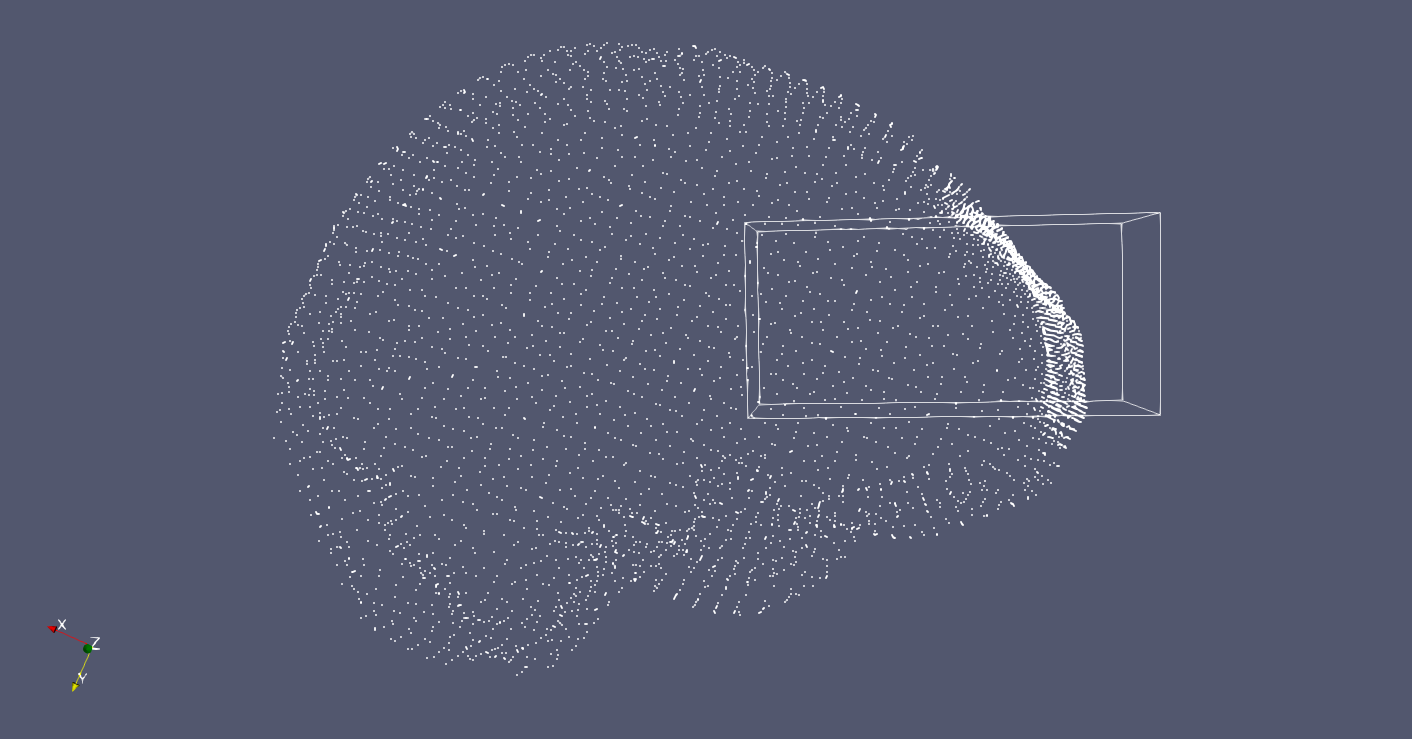
\includegraphics[width=1.0\textwidth]{figures/bad_quality_zone/cortex_surf.png}
        \caption{Perspectiva lateral}
    \end{subfigure}
    \begin{subfigure}[t]{0.45\textwidth}
        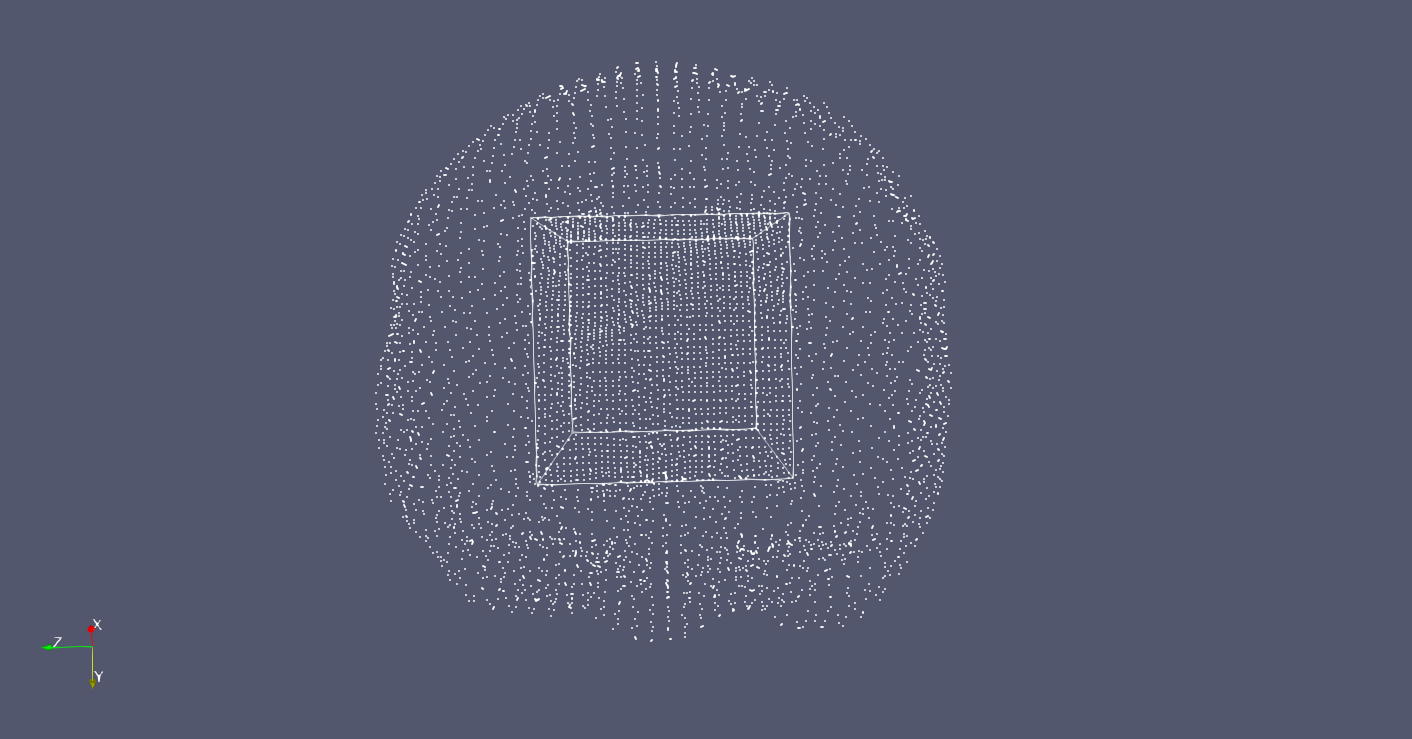
\includegraphics[width=1.0\textwidth]{figures/bad_quality_zone/cortex_surf_points.png}
        \caption{Perspectiva frontal}
    \end{subfigure}
    \caption{  Muestra frontal y lateral de la malla inicial con refinamiento global de nivel 5 y refinamiento en superficie prismática regular de nivel 7.\\ Fuente: Elaboración propia.}
    \label{fig:cortex_surf}
\end{figure}

\subsection{Herramientas}

En este trabajo se utilizarán algunas herramientas construidas por la comunidad como el generado de Mallas, el generador de estadísticas $J_{ENS}$, un software para visualización, scripts en Bash y Python para la ejecución de la solución y el análisis de los resultados, respectivamente.

\subsubsection{Mixed-element mesh generator} \label{section:mesh_generator_definition}

El generador de mallas de elementos mixtos \cite{lobos2015mixed} es una herramienta creada para facilitar la generación de mallas, a través de la linea de comandos se puede generar mallas con superficies de refinamiento en diferentes niveles, exportar en diversos formatos para visualización, iniciar con una malla refinada y refinar específicamente octantes entregados como input.
Este software recibe modelos de datos de mallas en formato \textit{mdl}.

\begin{lstlisting}[style=Console,caption={Opciones de mesher generator.\\ Fuente: Elaboración propia.}]
input  >    ./mesher -h
output >    use:  ./mesher [-d] input.mdl [-o] input.off [-u] output
                    [-c] volume_mesh.oct (octant mesh to start from)
                    [-s] ref_level [-a] ref_level [-b] file.reg 
                    [-l] list_file.txt [-r] input_surface rl [-g] [-v]
            where:
              one of the parameters must be an input surface mesh in
              mdl or off format. If output name is not provided it
              will be saved in input_name.m3d. Options:
                -s Refine octants intersecting the input surface.
                   Parameter ref_level is the refinement level
                -a Refine all elements in the input domain.
                   Parameter ref_level is the refinement level
                -b Refine block regions provided in file file.reg
                -l Refine elements provided in the file by their index
                -r Refine surface region. Will refine all the elements
                   in the provided input_surface at level rl
                -g save output mesh in GetFem format (gmf)
                -v save output mesh in VTK ASCII format (vtk)
                -i save output mesh in MVM ASCII format (mvm)
                -m save output mesh in M3D ASCII format (m3d)
\end{lstlisting}

Se denominará como \textit{MESHER\_GENERATOR} en el resto del presente trabajo.

\subsubsection{Mixed-element $J_{ENS}$ stadistics generator}

El generador de estadísticas $J_{ENS}$ para mallas Octree de elementos mixtos es una herramienta que facilita la validación de mallas, creada por la comunidad y liderado por el profesor Claudio Lobos. Puede generar histogramas con diferentes índices como Scaled Jacobian, Normalized Scaled Jacobian, Aspect Ratio, etc. 
En este trabajo lo utilizaremos principalmente para validar cada malla generada enfocándonos sólo en obtener la frecuencia del incide $J_{ENS}$. Esto es un histograma con la frecuencia de todos los elementos de la malla con $J_{ENS} \in \{-\infty , 1\}$, como se muestra en la figura \autoref{out:jens_output_c_5r7_0}.

\begin{lstlisting}[style=console,caption={Opciones de jens calculator. \\ Fuente: Elaboración propia.}]
input   >   ./jens -h
output  >   use: ./jacobian -option input.m3d
            options:
            -s : Scaled Jacobian statistics
            -e : Element Normalized Scaled Jacobian statistics
            -j : List Jens of each Element Jens [Js]
            -a : List Aspect Ratio for each element
            -l : List Jens of each node for each element
\end{lstlisting}


\begin{lstlisting}[style=console,label={out:jens_output_c_5r7_0},caption={Estadísticas Jens para malla inicial, muestra una lista de frecuencias para diferentes cotas superiores para la calidad Jens encontrada en la malla.\\ Fuente: Elaboración propia.}]
input   >   ./jens -e ./src/c_5r7.mdl
output  >   negative: 27
            <0.0333 : 4
            <0.05   :5
            <0.1    :13
            <0.15   :54
            <0.2    :219
            <0.25   :356
            <0.3    :9918
            <0.35   :8431
            <0.4    :3386
            <0.45   :6641
            <0.5    :2341
            <0.55   :16891
            <0.6    :2659
            <0.65   :2689
            <0.7    :2038
            <0.75   :4872
            <0.8    :1108
            <0.85   :2477
            <0.9    :457
            <0.95   :408
            <1      :108662
            total: 173656
            worst quality -0.792707
            average quality 0.806127
\end{lstlisting}

Se denominará como \textit{JENS\_CALCULATOR} en el resto del presente trabajo.

Convenientemente, los primeros tres intervalos del histograma pertenecen a los intervalos de interés para este estudio.

\subsubsection{ParaView}

Paraview es un software open-source multiplataforma que facilita la visualización de representaciones en 3D. Presenta una interfaz interactiva, nos ayudará analizar visualmente el estado de la malla en todo momento. Se utilizará el formato con extensión \textit{vtk} para visualizar mallas en esta plataforma.

Este software presenta diferentes secciones que nos ayudarán a analizar cada malla generada, la sección marcada con el número 1 en \autoref{fig:paraview_all}, se presentan todas las mallas que se representarán gráficamente en la sección 2. Existe un panel de herramientas en la sección 3 que nos ayudará a marcar/desmarcar elementos o puntos en el panel 2 que se verán reflejados e identificados en el recuadro 5.
En la sección 4 podremos cambiar la forma de visualizar cada representación, esto nos ayudará a identificar elementos, identificar si una malla es válida en su construcción, etc.

\begin{figure}[!ht]
    \centering
    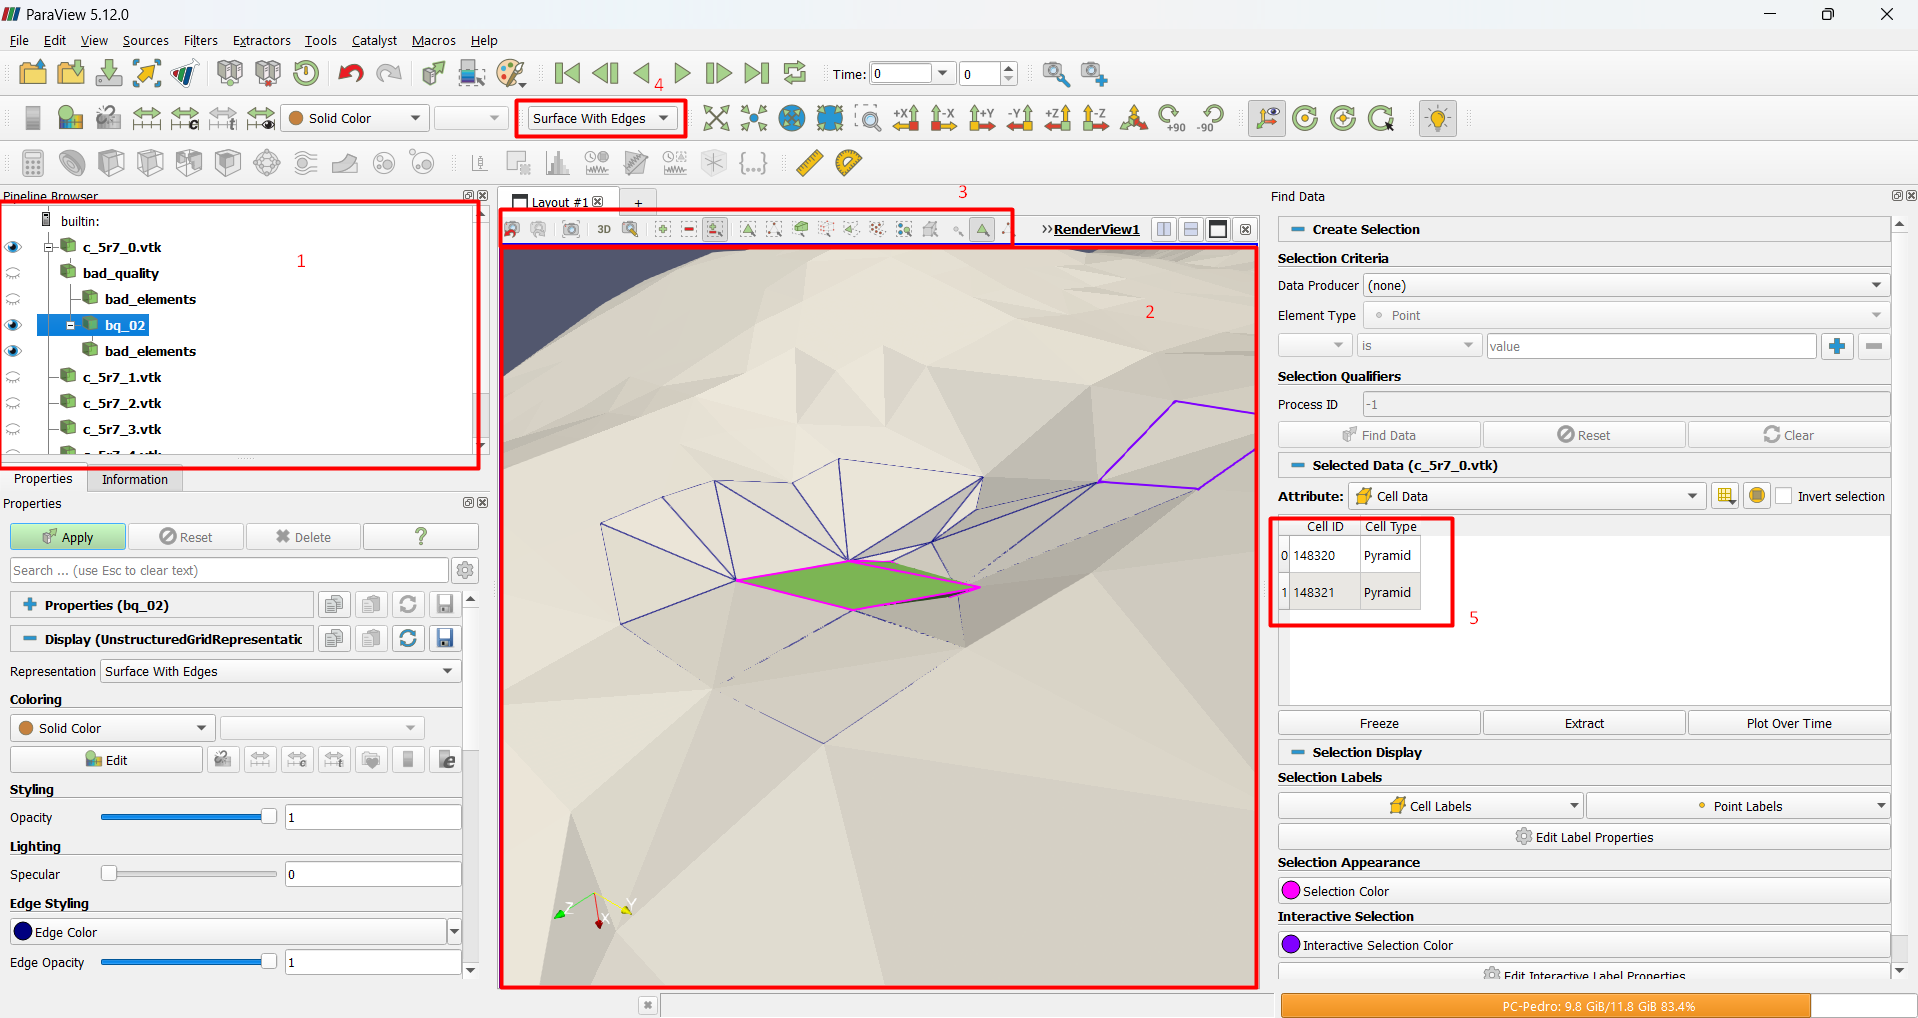
\includegraphics[width=1.0\textwidth]{figures/paraview/paraview_all.png}
    \caption{ Interfaz de software Paraview, se muestra una sección de la malla inicial con dos elementos seleccionados.\\  Fuente: Elaboración propia.}
    \label{fig:paraview_all}
\end{figure}

\subsection{Estructura de datos}

En la construcción de la solución existen diversas estructuras de datos que se van complejizando a medida que se avanza en el algoritmo.

En esta sección sólo se explicará la estructura de datos elemental y de forma general. 

Como se definió anteriormente, una malla Octree se divide en octantes, cada uno de estos octantes contienen Elementos mostrados en la \autoref{fig:basics_elements}.  Luego, cada uno de estos Elementos está constituido por Puntos, que es la unidad más pequeña.

Para ejemplificar en \autoref{fig:entity_relation_diagram}, se presenta un pequeño diagrama entidad relación que muestra la estructura de los objetos relacionados en el algoritmo de la generación de mallas.

%\begin{lstlisting}[style=CStyle,caption={Clase Octant.\\ Fuente: Elaboración propia.},label={code:octant_class}]
%#include <vector>
%class Octant
%{
%	public:
%        Octant(vector<unsigned int> &epts, const unsigned short &ref_level,
%    			   const unsigned int &o_id);
%        ...
%        // indice del octante.
%        unsigned int id;
%        // indices de puntos que conforman al octante.
%        vector<unsigned int> points_indexes;
%        // indices de puntos que conforman los elementos 
%        // pertencientes al octante.
%        vector<vector<unsigned int>> sub_elements_points_indexes;
%}
%\end{lstlisting}

\begin{figure}[!ht]
	\centering
	\includegraphics[width=0.8\textwidth]{figures/entity_relation_diagram.png}
	\caption{Diagrama entidad-relación de el generador de mallas.\\  Fuente: Elaboración propia.}
	\label{fig:entity_relation_diagram}
\end{figure}

\subsubsection{Acercamiento al algoritmo de Mixed-element mesh generator}

Parte importante del software mencionado en la Sección \ref{section:mesh_generator_definition} es la generación de la malla que se define y explica brevemente en \cite{daines2018repairing}.


\begin{algorithm}
\SetKwInOut{KwIn}{Input}
\SetKwInOut{KwOut}{Output}
% functions
\SetKwFunction{generateMesh}{GENERATE\_MESH}
\SetKwFunction{generateBalancedOctree}{GENERATE\_BALANCED\_OCTREE}
\SetKwFunction{applyTransitionPatterns}{APPLY\_TRANSITION\_PATTERNS}
\SetKwFunction{applySurfacePatterns}{APPLY\_SURFACE\_PATTERNS}
\SetKwFunction{projectOnto}{PROJECT\_ONTO}
\SetKwFunction{add}{ADD}
\SetKwFunction{getBoundaryNodes}{GET\_BOUNDARY\_NODES}
% procedure
\SetKwProg{myproc}{Procedure}{:}{}
\KwIn{Refinement level constraints $RLC$, triangular surface mesh \Omega.}
\KwOut{Volumetric mesh of \Omega that meets $RLC$.}
\myproc{\generateMesh{RLC, \Omega}}
{
    $mesh$ \gets \generateBalancedOctree{RLC,\Omega}\;
    $mesh$ \gets \applyTransitionPatterns{mesh}\;
    $bnodes$ \gets \getBoundaryNodes{mesh, \Omega}\;
    \For{ \textbf{each} $node$ \textbf{in} $bnodes$} {
        \If{$node \in l$ \textbf{or} ($node$ is \textbf{inside} of \Omega\, \& $node$ is \textbf{close} to \Omega)} {
            $node$.\projectOnto{\Omega}\;
        }
    }
    $mesh$ \gets \applySurfacePatterns{mesh}\;
    $bnodes$ \gets \getBoundaryNodes{mesh, \Omega}\;
    \For{\textbf{each} $node$ \textbf{in} $bnodes$} {
        \If{$node$ is \textbf{outside} of \Omega} {
            $node$.\projectOnto{\Omega} \;
        }
    }
    \KwRet mesh\;    
}
\caption{Algoritmo de generación de mallas Octree con elementos mixtos y varios niveles de refinamiento.\\ Fuente: \cite{daines2018repairing}}
\label{alg:propuesta_daines} 
\end{algorithm}

Es importante además explicar brevemente los diferentes formatos de exportación del algoritmo.
%Esto porque se utilizarán para mantener un historial de
% .histo, .m3d, .map, .oct, .ref


